\documentclass[a4paper,12pt]{article}

% Codificación y lenguaje
\usepackage[utf8]{inputenc}
\usepackage[T1]{fontenc}
\usepackage[spanish]{babel}
\usepackage[utf8]{inputenc}

% Paquetes esenciales
\usepackage{graphicx}
\usepackage{geometry}
\usepackage{datetime}
\usepackage{titlesec}
\usepackage{fancyhdr}
\usepackage{parskip}
\usepackage{array}
\usepackage{float}
\usepackage{placeins}
\usepackage{hyperref}
% Paquetes para código fuente
\usepackage{listings}
\usepackage{xcolor}

% Configuración del estilo de listings para código Arduino
\lstdefinestyle{arduino}{
  language=C++,
  basicstyle=\ttfamily\footnotesize,
  keywordstyle=\color{blue},
  commentstyle=\color{gray},
  stringstyle=\color{red},
  numbers=left,
  numberstyle=\tiny,
  stepnumber=1,
  numbersep=5pt,
  backgroundcolor=\color{white},
  frame=single,
  breaklines=true,
  captionpos=b
}
\lstset{style=arduino}

% Márgenes del documento
\geometry{left=3cm, right=2.5cm, top=3cm, bottom=3cm}

\begin{document}

% Incluir carátula (asegurate de que caratula.tex exista)
\begin{titlepage}
    \begin{center}
        {\LARGE \textbf{Universidad Nacional de Córdoba}}\\[1.5cm]

        
\includegraphics[scale=0.4]{img/logo2.png}\\[1.5cm]

        {\large Facultad de Ciencias Exactas, Físicas y Naturales}\\

        \rule{\linewidth}{0.5mm}\\[0.4cm]
        {\Large \textbf{Cátedra de Arquitectura de Computadoras}}\\[0.3cm]
        {\LARGE \textbf{Trabajo Práctico 1: ALU}}\\[0.3cm]
        \rule{\linewidth}{0.5mm}\\[1cm]

        \begin{flushleft}
        {\large 
            \textbf{Profesores:} - Martin Pereyra, Santiago Rodriguez\\
            \textbf{Integrantes:}\\
            Pallardó Agustín - 
            \href{mailto:apallardo@mi.unc.edu.ar}{apallardo@mi.unc.edu.ar}\\
            Trachta Agustín - 
            \href{mailto:agutrachta@mi.unc.edu.ar}{agutrachta@mi.unc.edu.ar}\\
        }
        \end{flushleft}

        \vfill

        {\large \today}
    \end{center}
\end{titlepage}


\tableofcontents
\clearpage

\section{Introducción}
En este informe se documenta el desarrollo de una Unidad Aritmético-Lógica (ALU) implementada en una FPGA Basys 3.  
La ALU constituye un bloque fundamental en el diseño de procesadores y sistemas digitales, ya que permite realizar operaciones aritméticas, lógicas y de desplazamiento sobre datos binarios.  

El objetivo principal de este trabajo práctico es adquirir experiencia en la descripción de hardware mediante Verilog, la validación con bancos de prueba, la simulación usando la herramienta Vivado, y la implementación física real.

\section{Objetivo}
Los objetivos específicos del trabajo práctico son:  
\begin{itemize}
    \item Implementar una ALU parametrizable en Verilog, de modo que el ancho del bus de datos pueda ajustarse según futuras necesidades.
    \item Validar la implementación mediante un banco de pruebas (\textit{testbench}) que genere entradas asignadas y contemple un mecanismo de validación.
\end{itemize}

Las operaciones que soportará la ALU son las siguientes:  
\begin{center}
\begin{tabular}{|c|c|}
\hline
\textbf{Operación} & \textbf{Código}\\
\hline
ADD & 100000 \\
SUB & 100010 \\
AND & 100100 \\
OR  & 100101 \\
XOR & 100110 \\
SRA & 000011 \\
SRL & 000010 \\
NOR & 100111 \\
\hline
\end{tabular}
\end{center}

\section{Desarrollo}
Para la implementación del proyecto se ha creado un módulo de Verilog \textbf{alu.v} que contiene las operaciones mencionadas anteriormente, y otro módulo \textbf{top.v} que instancia la ALU y que se utilizará para conectar sus entradas y salidas a los pines físicos de la FPGA mediante los constraints, además de generar los registros necesarios para poder realizar las pruebas.

\section{Diagrama en bloques de la arquitectura}
En la Figura~\ref{fig:diagrama} se presenta el diagrama en bloques de la ALU.

\begin{figure}[H]
    \centering
    % 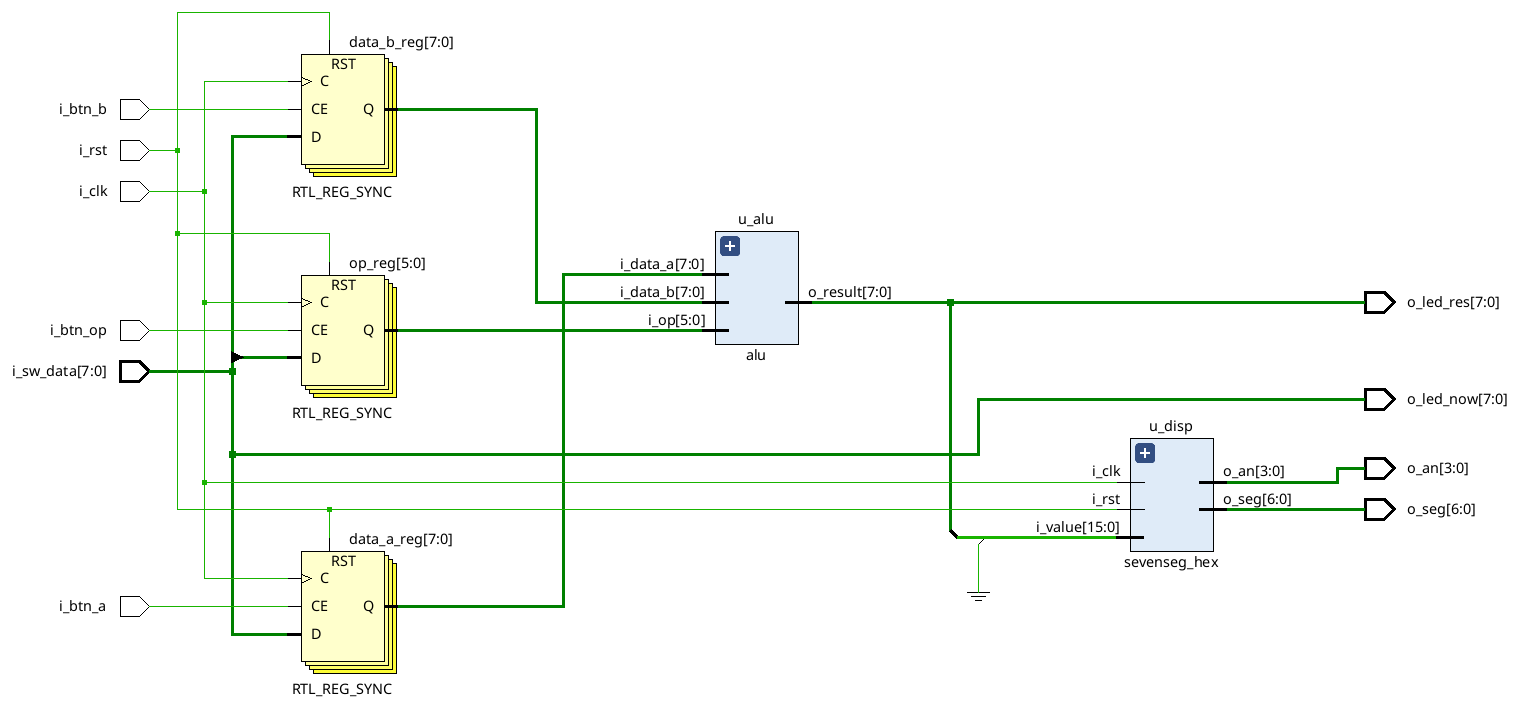
\includegraphics[width=0.7\textwidth]{diagrama.png}
    \caption{Diagrama en bloques de la arquitectura de la ALU.}
    \label{fig:diagrama}
\end{figure}

\section{Imágenes de la simulación}
En esta sección se observan capturas obtenidas en la herramienta Vivado.

\begin{figure}[H]
    \centering
    % 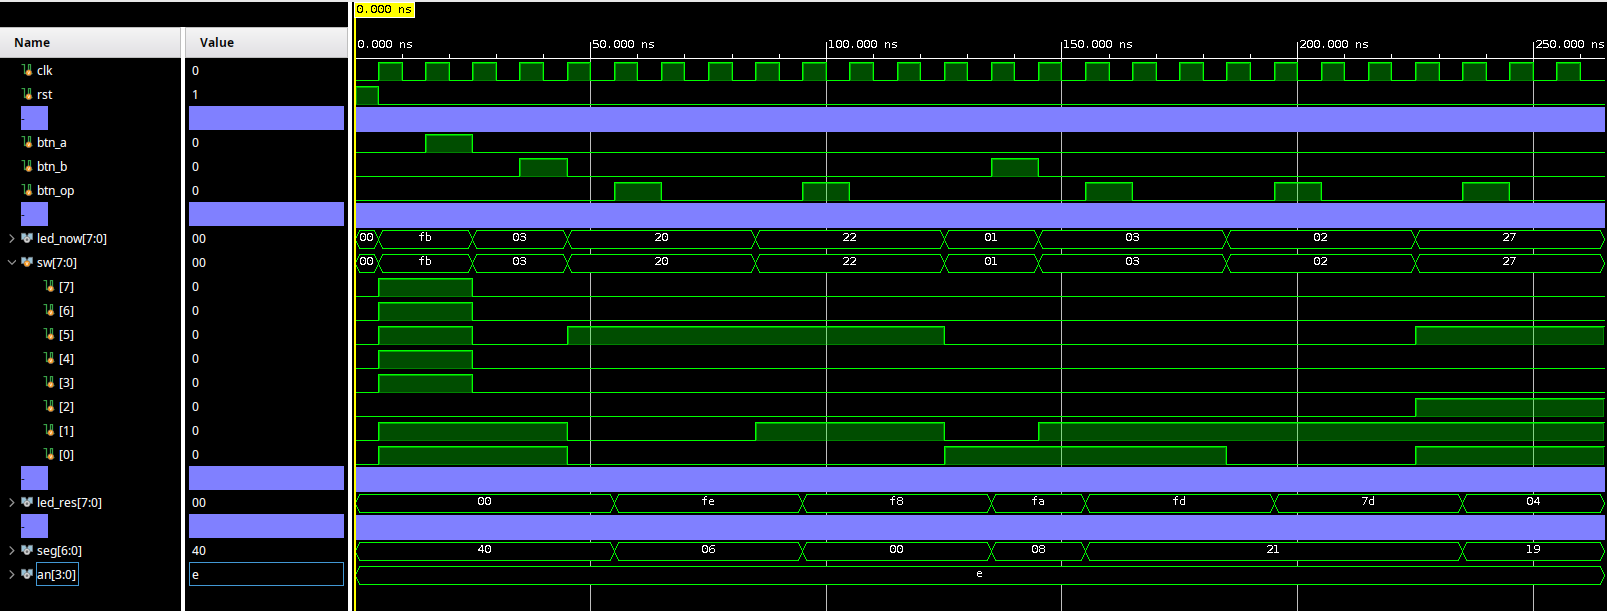
\includegraphics[width=0.8\textwidth]{simulacion.png}
    \caption{Ejemplo de simulación en Vivado.}
\end{figure}

\section{Repositorio del proyecto}
El código fuente, los archivos de simulación y los bancos de prueba se encuentran disponibles en el siguiente repositorio:  

\href{https://github.com/AguTrachta/ComputerArchitecture/tree/develop/ALU}{https://github.com/AguTrachta/ComputerArchitecture/tree/develop/ALU}

\end{document}